\chapter{Resultados}
\label{cap:resultados}

% todo

% todo analise exploratoria
\section{Análise Exploratoria}
\label{cap:resultados:sec:analise_exploratoria}

Antes de iniciarmos a analise de sentimento podemos encontrar informações interessantes utilizando tecnicas mais simples de processamento de linguagem natural.

Após devido tratamento das avaliações conseguimos obter as nuvens de palavras considerando todas as palavras \ref{wordcloud_geral}, onde podemos notar como alguns dos destaques quarto, piscina, praia, restaurante, como sendo as palavras com maior frequência nas avaliações.


Já considerando a nuvem de palavras filtrando apenas por adjetivos teremos então \ref{img:wordcloud_adjetivos} que tem como alguns dos destaques palavras como sensacional, execelente, especial, local, top, otimo, nota.

E por ultimo observamos a nuvem de palavras levando em consideração apenas os substantivos \ref{img:wordcloud_substantivos}, que como destaque podemos citar funcionario, piscina, quarto, praia.

Uma outra forma de analise é o agrupamento de tokens em unigramas \ref{img:unigramas}, bigramas \ref{img:bigramas} e os trigramas \ref{img:trigramas} presentes em todas as avaliações. dessa forma temos exatamente a classificação de frenquencia dos tokens no corpus de estudo.

Entre os unigramas \ref{img:unigramas} temos uma lista com alguns dos tokens mais frequêntes, alguns chegando a passar a contagem de utilização de mais de 10.000 vezes, como é o caso de lugar, sendo seguindo ainda que proximo por comida, excelente e atendimento, este ultimo com uma frequência próximo de 8500 vezes. Ainda em relação aos unigramas também podemos levar em consideração a sua frequência com a evolução do tempo em \ref{img:rank_unigramas}, e algo com grande destaque é a palavra lugar que está entre o top 10 entre todo o periodo da analise, flutuando entre as cinco primeiras posições, tio é um unigrama que merece atenção, por não ter aparecido na nuvem de palavras de unigramas, porém se faz presente no ranking se observarmos individualmente os anos ele aparece em décimo lugar no ano de 2022, indicios de uma possivel atração local bem conhecida, substituindo então o unigrama 'praia', que se fazia presente no ranking até 2021 na nona colocação.

Considerando os bigramas \ref{img:bigramas} a frequência diminui consideravelmente, pois aqui temos que a ordem importa e dessa forma o mais frenquênte fica proximo de 1700 vezes, sendo composto pela dupla 'lugar' e 'maravilhoso', seguido pelo segundo colocado, bem próximo de 1400 vezes, sendo 'comida' e 'boa', onde podemos observar a grande frequência de palavras positivas, por conta dos adjetivo positivos.

Para destaque entre os trigramas \ref{img:trigramas} a frequência diminui ainda mais e como destaque tmos um que supera a contagem de 250 vezes, sendo 'facilidade', 'deslocamento' e 'pe', o que nos indica que existe pelo menos um hotel que possui uma boa localizacao para que seja possivel se deslocar até uma atração popular do local à pé, seguido de 'atendimento', 'nota' e '10' que indica que para as pessoas que avaliaram o atendimento da rede de hotéis ainda é algo importante e que deve ser levado em consideração caso a rede tenha interesse em ter ou manter um conceito positivo entre seus cliente.


\begin{figure}
	\centering
	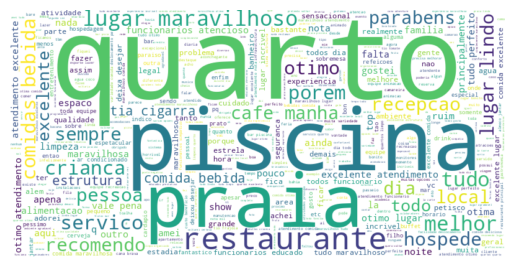
\includegraphics[width=1\textwidth]{figs/exploratoria/wordcloud_geral.png}
	\caption{Wordcloud sem stop words}
	\label{img:wordcloud_geral}
\end{figure}


\begin{figure}
	\centering
	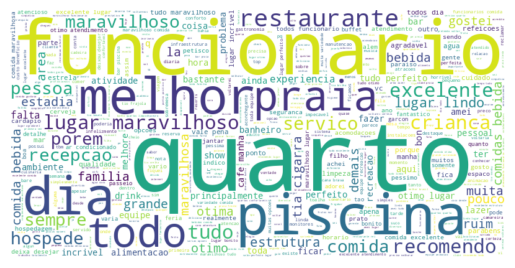
\includegraphics[width=1\textwidth]{figs/exploratoria/wordcloud_substantivos.png}
	\caption{Wordcloud de substantivos}
	\label{img:wordcloud_substantivos}
\end{figure}

\begin{figure}
	\centering
	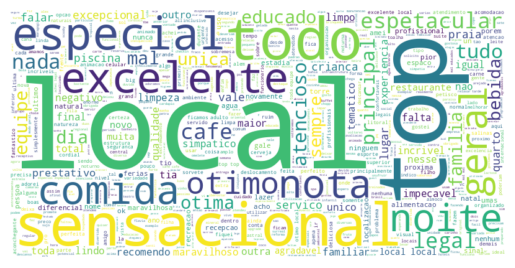
\includegraphics[width=1\textwidth]{figs/exploratoria/wordcloud_adjetivos.png}
	\caption{Wordcloud de Adjetivos}
	\label{img:wordcloud_adjetivos}
\end{figure}

\begin{figure}
	\centering
	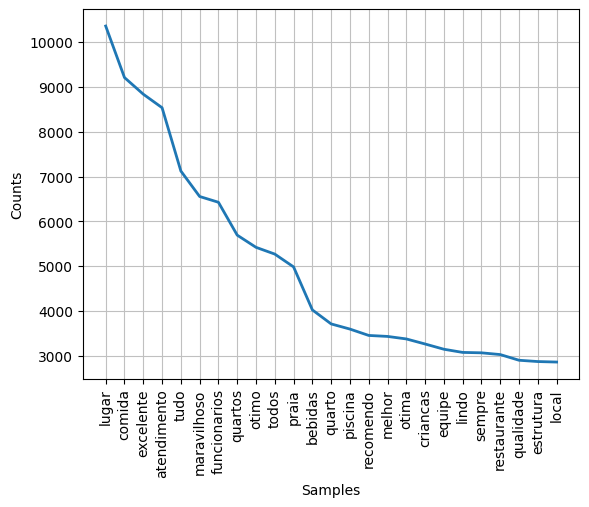
\includegraphics[width=1\textwidth]{figs/exploratoria/unigramas.png}
	\caption{Unigramas}
	\label{img:unigramas}
\end{figure}

\begin{figure}
	\centering
	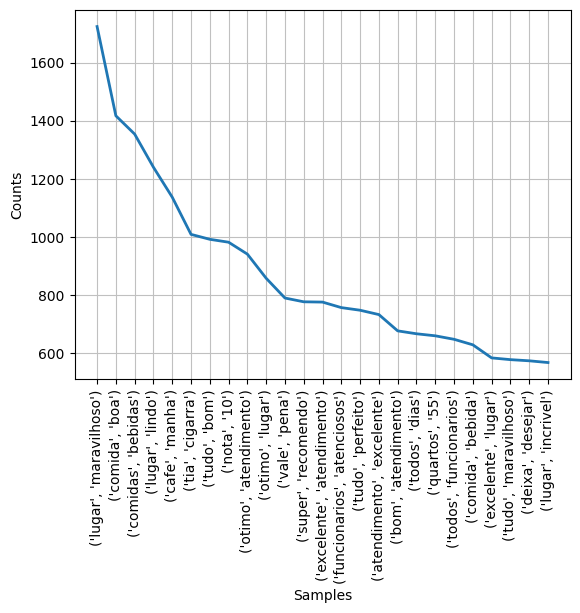
\includegraphics[width=1\textwidth]{figs/exploratoria/bigramas.png}
	\caption{Bigramas}
	\label{img:bigramas}
\end{figure}

\begin{figure}
	\centering
	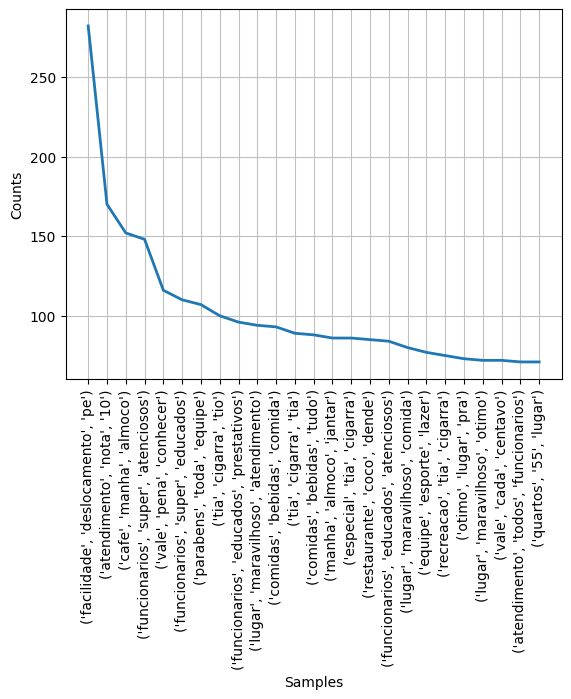
\includegraphics[width=1\textwidth]{figs/exploratoria/trigramas.png}
	\caption{Trigramas}
	\label{img:trigramas}
\end{figure}


%TODO ajustar tamano, ta estranho
\begin{figure}
	\centering
	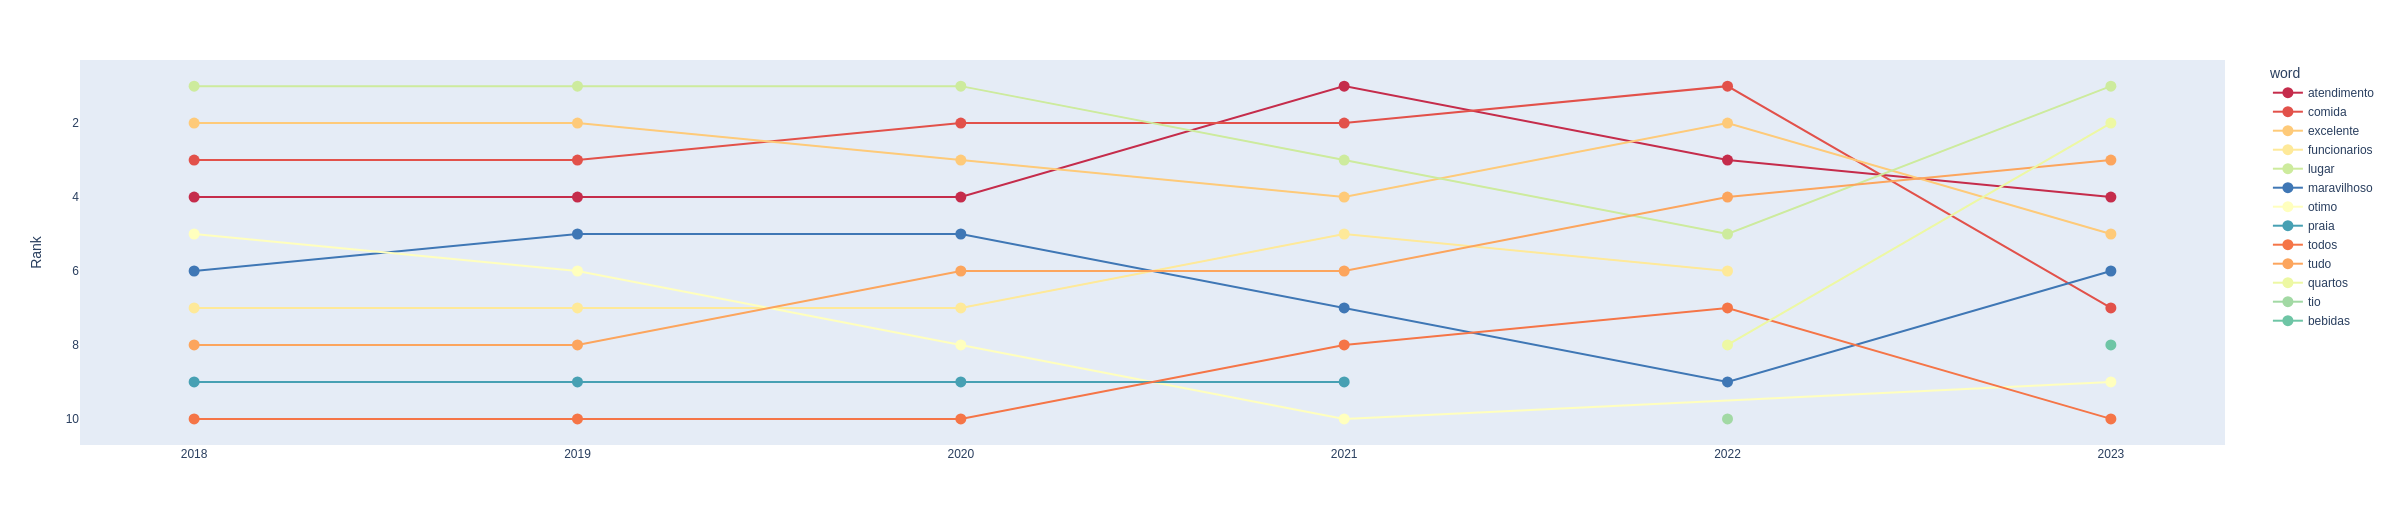
\includegraphics[width=.7\textwidth]{figs/exploratoria/ranking_unigramas_por_ano.png}
	\caption{Ranking de unigramas por ano}
	\label{img:rank_unigramas}
\end{figure} fgs

\section{Análise de Sentimentos}
\label{cap:resultados:sec:analise_sentimento}

Utilizando o modelo GPT 3.5 para realizar a tarefa de analise de sentimentos do conteudo textual das avaliações obtemos a distribuição conforme \ref{img:gpt_pizza_distribuicao}, onde 84.77\% das avaliações, ou seja, 41721 avaliações foram classificadas como tendo um sentimento positivo, isso representa um número próximo das avaliações que receberam como nota 4 ou 5, 6128 e 38347 avaliações respectivamente, porém fica facil notar em \ref{gpt_sentimento_nota} que mesmo a grande maioria das avalições com essa nota atribuida ainda existem avaliações com sentimentos diferentes

\begin{figure}
	\centering
	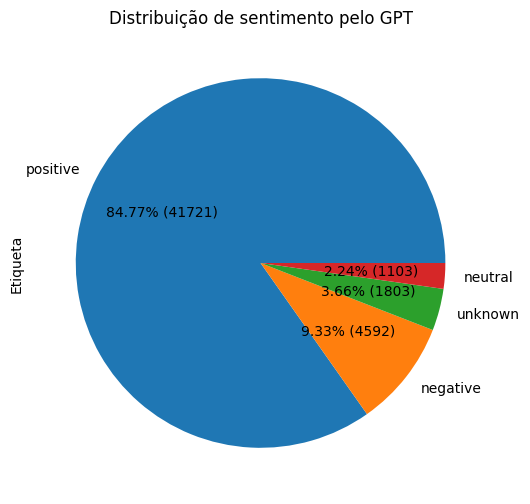
\includegraphics[width=1\textwidth]{figs/gpt/distribuicao_pizza.png}
	\caption{Distribuição do sentimento das avaliações}
	\label{img:gpt_pizza_distribuicao}
\end{figure}

\begin{figure}
	\centering
	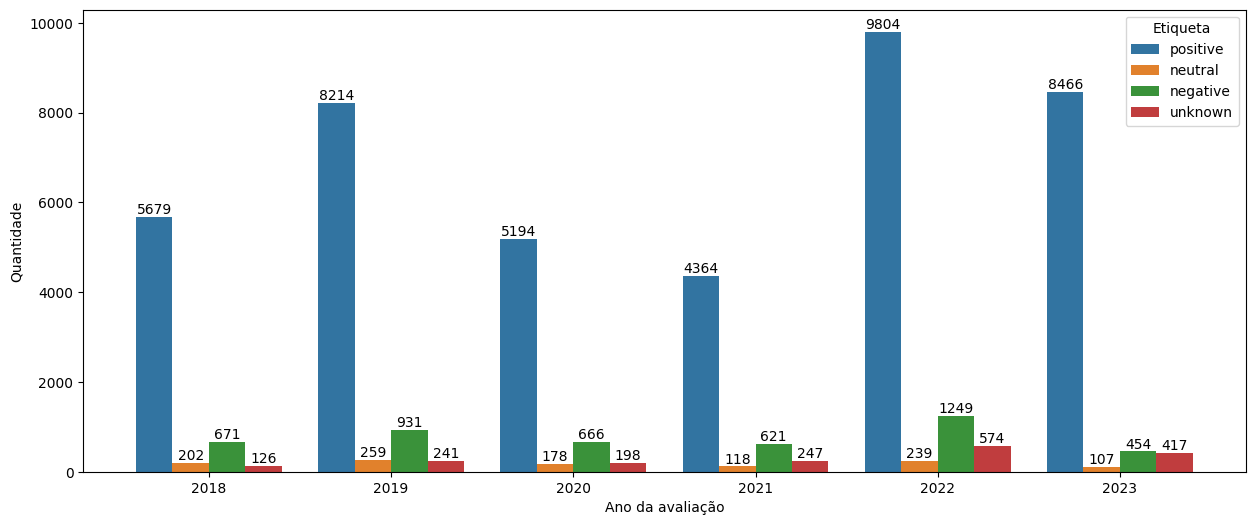
\includegraphics[width=1\textwidth]{figs/gpt/sentimento_ano.png}
	\caption{Sentimento das avaliações por ano}
	\label{img:gpt_sentimento_ano}
\end{figure}

\begin{figure}
	\centering
	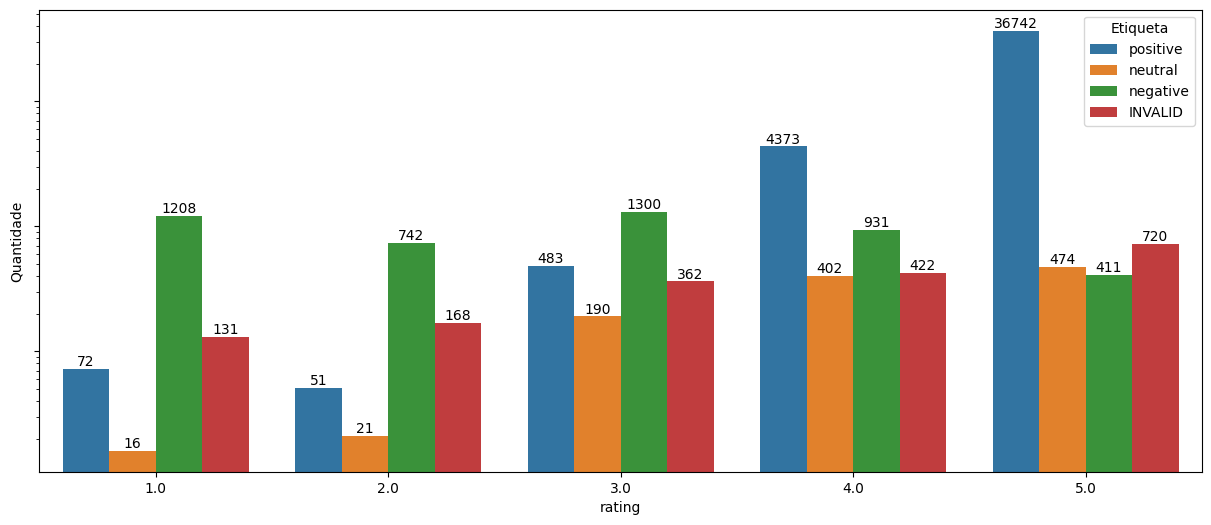
\includegraphics[width=1\textwidth]{figs/gpt/sentimento_nota.png}
	\caption{Sentimento das avaliações por nota}
	\label{img:gpt_sentimento_nota}
\end{figure}



% E dentre todas as avaliações obtidas utilizaremos para a analise o total de 49219(57.04\%) e 37072(42.96\%) foram ignoradas

% sentimento bert

% sentimento gpt

% sentimento temporal

% outros LLMs

% bert vs GPT

% inconsistencias? revalidaçoes?
